
\documentclass[twocolumn]{article}
\usepackage{mathpazo}
\usepackage{microtype}
\usepackage{times}
\usepackage{titlesec} % 1
%\usepackage{sectsty} % "제 1 절" ...

 %%%%%%%%%%%%%%%%%%%%%%%%%%%%%%%%%%%%%%%%%%%%%%%%%%%%%%%%%%%%%%%%%%%%%%%%%%%%%
 %                              My Commands
\newcommand{\bi}{\begin{itemize}}
\newcommand{\ei}{\end{itemize}}
\newcommand{\be}{\begin{enumerate}}
\newcommand{\ee}{\end{enumerate}}
\newcommand{\ii}{\item}
\newtheorem{Def}{Definition}
\newtheorem{Lem}{Lemma}
\usepackage{algorithm}
\usepackage{algorithmicx}
\usepackage{algpseudocode}

\usepackage{graphicx}
\graphicspath{%
        {converted_graphics/}
        {./images/}
}

\usepackage[hangul,nonfrench,finemath]{kotex}
    
\setlength\textwidth{7in} 
\setlength\textheight{9.5in} 
\setlength\oddsidemargin{-0.25in} 
\setlength\topmargin{-0.25in} 
\setlength\headheight{0in} 
\setlength\headsep{0in} 
\setlength\columnsep{9pt}
\sloppy 
 
\begin{document}

\title{
\vspace{-0.5in}\rule{\textwidth}{2pt}
\begin{tabular}{ll}\begin{minipage}{4.75in}\vspace{6px}
\noindent\large {\it KIWI Project}@Data Management Research Section\\
\vspace{-12px}\\
\noindent\LARGE ETRI\qquad  \large Technical Report 14ZS1410-TR-61
\end{minipage}&\begin{minipage}{2in}\vspace{6px}\small
218 Gajeong-ro, Yuseong-gu\\
Daejeon, 305-700, South Korea\\
http:/$\!$/www.etri.re.kr/\\
http:/$\!$/sungsoo.github.com/\quad 
\end{minipage}\end{tabular}
\rule{\textwidth}{2pt}\vspace{0.25in}
\LARGE \bf 구글 파일 시스템 \\
\large The Google File System
}

\date{}

\author{
{\bf Sung-Soo Kim}\\
\it{sungsoo@etri.re.kr}
}

\maketitle

\begin{abstract}
{\small
구글 파일 시스템은 대용량 분산 데이터전문 어플리케이션을 위한 유연한 분산파일 시스템으로,  저가의 일반적인 하드웨어 상에서 동작하면서도 무정지 기능(failure tolerance)과 많은 수의 클라이언트에 대한 높은 군집성능(high aggregate performance)을 제공한다.

 이러한 시스템설계의 기능상 목표는 기존의 분산 파일시스템들과  많은 부분이 공통되지만, 선행 파일시스템들의 예측과의 결정적인 차이점으로, 우리는 현재, 그리고 앞으로 예측되는 어플리케이션의 부하(workload)와 기술적 환경에 중점을 두고 설계하려고 노력했고,  이로 인해  전통적인 시스템디자인 방식을 재검토하고 근본적으로 다른 디자인컨셉을 시도하게되었다.

  이 파일 시스템은 우리가 필요로했던 저장기능을 성공적으로 수행했으며 구글의 주 저장 플랫폼으로 채택되어 오랫동안 구글 서비스뿐만 아니라 대량의 데이터 셋을 요구하는 연구와 개발 분야에 사용되었다.  이중 가장 큰 클러스터는 수천개의 디스크에 걸쳐 구성된 수백 테러바이트의 사이즈를 가지며 동시에 수백명의 클라이언트에 의해 접속되고 있다.

 여기서는 분산 어플리케이션을 지원하기 위해 설계된 파일 시스템 인터페이스 확장을 소개하고, 이 설계의 다양한 측면과 실제 상황과 이론상의 벤치마크결과에 대해 이야기하려고 한다.
}
\end{abstract}

\section{Introduction}

%\begin{figure}[!t]
%        \centering
%        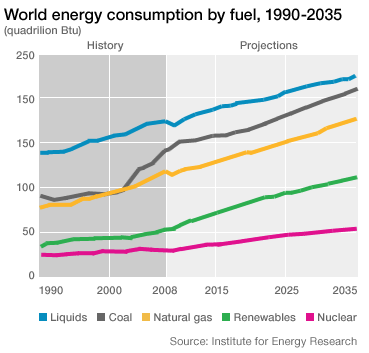
\includegraphics[width=0.33\textwidth]{test}
%        \caption{Caption}
%        \label{fig1}
%\end{figure}

 구글 파일 시스템(GFS)은 급속히 늘어나는 구글의 데이터 처리양을 해결하기 위해서 설계되었다 \cite{Ghemawat:2003:GFS, Ghem:2003:GFS}.  GFS의 특징인 성능, 확장성, 안정성, 유용성등은 기존의 분산파일 시스템과 유사하다고 볼수 있으나,  기존 시스템과의 결정적인 차이는 GFS는 현재 그리고 예측가능한 미래의 어플리케이션 부하와 기술 환경에 대한 관측을 통해서 전통적인 방식들을 재 검토하고 설계에 대해서 근본적으로 다른 시점으로 설계했다는 점에 있다.

 우선, 구성요소(component)의 오류는 당연하다고 간주한다.  파일시스템은 수백 혹은 수천개의 저가용 하드웨어로 구성된 저장 기기에서 구현되며 상당한 숫자의 클라이언트에서 접속된다.  이러한 구성요소의 양과 질을 감안하면, 어느 시점에서건 구성요소중 일부는 작동하지 않고 일부는 복구 불가능한 상태에 빠져있다고 가정해도 틀리지 않을것이다.  이러한 원인으로는 어플리케이션의 버그, OS상의 버그, 사용자 실수 혹은 디스크,메모리,연결단자,네트웍, 전원쪽의 오류등 다양한 가능성이 있다.  그러므로 이러한 시스템에는 지속적인 모니터링과 오류검사, 무정지 기능 그리고 자동 복구기능이 필수적이다.

 다음으로 고려할것은 기존에 비해 훨씬 증가한 파일들의 크기이다.  이들은 하나가 몇 기가인 경우가 일반적이고 웹 문서와 같은 파일은 대부분 여러 어플리케이션 객체를 포함하고 있기까지 한다.  몇억개의 객체로 구성된 수 테라 단위의, 빠르게 사이즈가 증가하고 있는 데이터를 일상적으로 다루어야 하는 환경이라면, 이를 킬로바이트 단위의 수 억개 객체로 관리하는 것은 효율적이지 못하다.  그래서 GFS의 설계는 입출력 작업과 블록 크기에 대한 기존의 상식을 재검토해야만 했다.

 세번째 고려사항은 대부분의 파일이 새로운 데이터에 의해 덮어쓰여지는 것이 아니라 추가확장되어간다는 점이다.  파일 내의 임의의 위치에 마음대로 쓰기를 할수 있는 기술은 실재로는 구현하지 않는다.  한번 작성된 파일은 단순히 읽기만 가능하며 대부분 순차적으로만 읽혀진다.  이러한 특성을 갖는 데이터의 종류는 매우 다양하다.  거대한 저장구역(repository)을 지정하여 데이터 분석 프로그램이 검색할수 있도록 하는 경우라던가, 수행되고 있는 어플리케이션에서 계속해서 생성되는 데이터스트림이라던가, 보관되어있는 데이터 혹은 하나의 머신에서 나온 결과가 다른 머신에서 수행되기 전의 중간결과들이 이에 해당한다.  이러한 파일접근방식이 대용량의 파일에 적용된다고 가정하면, 기능 향상과 원자성 보장(atomicity guarantee)을 위해서 중점을 두어야 할 부분은 클라이언트의 데이터 블록 캐슁 알고리즘이 아니라 파일의 확장(appending) 알고리즘이라는 것을 알수 있다.

  네번째로, 어플리케이션과 파일 시스템 API를 같이 설계한다는 것은 유연성 측면에서 전체 시스템의 효율을 높여준다.  예를 들어, 느슨한 GFS의 일관성 규약(consistency model)덕분에  어플리케이션 쪽에 귀찮은 여러 제약을 부가하지 않고 대단히 단순화된 파일 시스템을 구현할수 있었다.  또한 아토믹 어펜드 (atomic append) 기능은 별도의 동조화(synchronization)를 필요로 하지 않고도 복수의 클라이언트가 동시에 하나의 파일에 추가할수 있도록 한다.

  현재 다양한 GFS 클러스터들이 서로 다른 목적을 위해 구성되어 있으며, 가장 큰 클러스터는 1000개 이상의 저장 노드와 300테라 이상의 디스크 저장영역을 가지고 서로다른 기기에서 수백의 클라이언트에게 끊임없이 이용되고 있다.

\section{Design Overview}
\subsection{Assumptions}

 이러한 필요성에 의한 설계에서 우리는 매우 창의적이고 도전적인 가정에 도달하게 되었다.  앞서 언급한 주요 고려사항에 대해서 좀더 자세히 설명하면;
\bi
\ii 시스템은 오동작이 수시로 발생하는 다수의 저가형 기기로 구성된다.  이 시스템은 지속적으로 자신을 모니터하며 구성요소의 오동작에 관계없이 동작하며 이를 검진, 복구할 수 있어야 한다.
\ii 시스템은 적당한 수의 대용량 파일을 저장한다.  각각 100메가바이트 혹은 그 이상되는 수백만개의 파일을 기준으로 하되 기가바이트 단위의 파일들도 효율적으로 관리되어야 한다.  저용량 파일도 지원되야 하나 그런 파일을 위해 최적화될 필요는 없다.
\ii 시스템에 걸리는 부하는 대량 스트리밍 읽기와 소량 랜덤 읽기, 두종류의 읽기 동작이 주가 된다.  대량의 스트리밍 읽기에서는 각각의 동작(operation)이 수백 킬로바이트 혹은 1메가바이트 이상을 읽어들이게 되고, 동일한 클라이언트에 의한 연속되는 동작은 주로 그 파일의 연장영역에서 읽어오게 된다.  소량의 랜덤 읽기는 임의의 좌표에서 수 킬로바이트단위를 읽게 된다.  속도가 중요한 어플리케이션의 경우엔 대부분, 매번 앞뒤로 읽기 작업을 행하는 것 보다 여러 랜덤 읽기 작업을 모아서 정렬후 일괄적으로 읽어들이는 방식을 취한다.
\ii 부하에는 또한 파일에 데이터를 추가하는 대량의 순차적 쓰기도 포함된다.  일반적인 작업 크기는 읽기의 경우와 유사하다.  한번 쓰여진 파일은 다시 수정되는 경우가 매우 적으며,  임의의 위치에 소량의 데이터를 써넣는 기능은 지원되지만 효율적일 필요는 없다.
\ii 시스템은 반드시 복수의 클라이언트가 동일한 파일에 동시에 자료를 추가하는 것을 지원하도록 명확히 정의된 언어체계를 갖추고 있어야 한다.  이러한 파일들은 종종 제작자와 소비자 사이의 연결고리(queue)나 다방향 병합(many-way merging)에 사용된다.
\ii 신속한 반응속도(low latency) 보다는 고부하를 견뎌낼수 있는 대역(bandwith) 유지가 더 중요하다. 실제 대상이 되는 어플리케이션은 일부 개개 요청에 대한 응답시간을 엄격히 지켜야 하는 경우를 제외하고 대부분 데이터를 대용량 고속처리하는것에 더 큰 비중을 두고 있다.
\ei

\subsection{Interface}

  GFS는  POSIX와 같은 표준 API를 보유하고 있지는 못하지만 어느정도 친숙한 파일 시스템 인터페이스를 제공한다.  파일들은 디렉토리에 계층적으로 정리되며 경로명으로 접근할 수 있다.  파일을 생성, 삭제, 열기, 닫기, 읽기와 쓰기를 위한 립반적인 작업들 역시 지원된다.

 또한, GFS는 스냅샷 기능과 레코드 추가 기능을 지원한다.  스냅샷은 파일이나 디렉토리 구조의 복사본을 간단히 만들 수 있는 기능을 제공하며 레코드 추가 기능은 복수의 클라이언트가 추가하려는 각 데이터의 내용을 보장하면서 동시에 모든 클라이언트가 하나의 파일에 그 데이터들을 추가할 수 있도록 해준다.  이런 구조는 여러 곳에서 생성된 결과보고서를 다방향 병합하는 경우나, 복수의 클라이언트가 파일을 잠그지 않고 (lock) 동시에 데이터를 추가해야 하는 생산자-소비자 연결에 사용될 수 있다.  우리는 이러한 형태의 파일들이야말로 거대 분산 어플리케이션의 구성에 필요불가결하다는 것을 발견했다.  
%스냅샷과 레코드 추가기능에 대해서는 3.4항과 3.3에 각각 다시 설명될 것이다.

\begin{figure*}[thb]
        \centering
        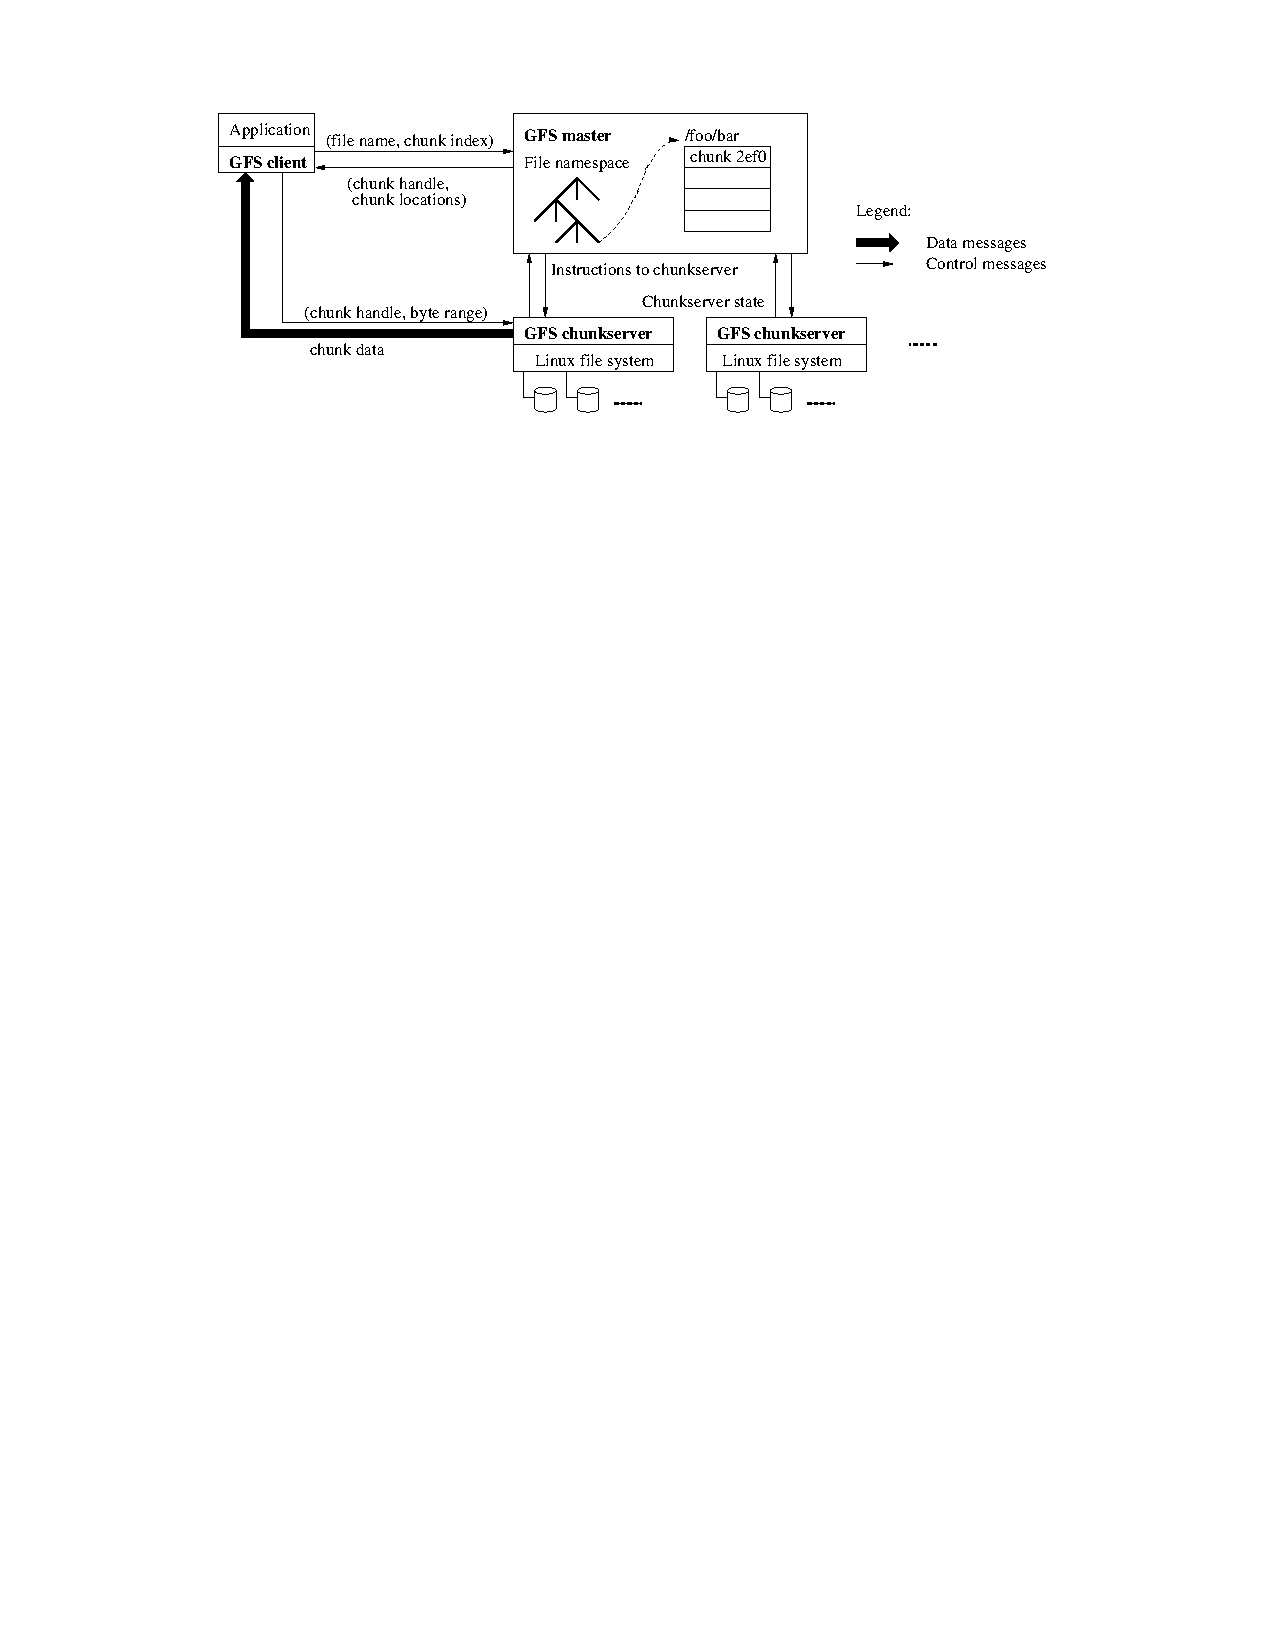
\includegraphics[width=0.8\textwidth]{architecture}
        \caption{GFS Architecture}
        \label{fig:architecture}
\end{figure*}

\subsection{Architecture}

  GFS 클러스터는 하나의 마스터와 여러개의 조각서버 (chunkserver) 로 구성되며, 그림 1과 같이 다중 클라이언트로부터 접근된다.  개개의 구성요소는 주로 사용자 레벨의 서버 동작을 하는 리눅스 기기이며 기기의 자원이 허용하는 한도 내에서라면 조각서버와 마스터를 하나의 서버에서 돌리는 것도 단순하게 구현된다.  물론 이경우 잘못된 어플리케이션 코드를 수행할 경우 안정성이 떨어질 수 있다.

 파일들은 고정된 크기의 조각(chunk)들로 나뉘어 저장된다.  각각의 조각은 서버 전체를 걸쳐 고유의 64비트 조각 번호 (chunk handle)을 마스터로부터 생성시 부여받게 되고 이 번호는 절대로 변경될 수 없다.  조각서버는 로컬 디스크에 조각들을 리눅스 파일로 저장하며 조각 번호와 해당 바이트 범위에 따라 파일을 읽고 쓰게 된다.  안정성 측면에서 각각의 조각은 여러 조각서버에 복사되는데, 기본 설정에서는 3개의 복사본을 저장하게 되며 사용자는 각각의 파일 네임스페이스 영역에 개별적인 복사 레벨을 지정할 수 있다.

 마스터는 모든 파일 시스템의 메타데이터를 관리한다.  여기에는 네임스페이스, 접근 조절 정보, 파일 조각 매핑과 각 조각의 현재 위치등이 포함되며, 마스터는 또한 조각 임대(lease) 관리, 연결이 유실된 조각(orphaned chunk)의 유휴메모리 정리 (garbage collection), 조각 서버들간의 조각 이동과 같은 시스템 수준 동작을 관리한다.  마스터는 주기적으로 각각의 조각서버와 맥박신호(heartbeat message)를 교환함으로써 명령을 전달하고 각 서버의 상태를 수집한다.

 GFS 클라이언트 코드는 이 파일시스템 API를 적용하고 있는 각각의 어플리케이션과 링크되어 어플리케이션전반에 걸친 마스터와 조각서버간의 통신에 관여하게 된다.  클라이언트는 마스터와 통신하며 메타데이터 관련 작업을 수행하지만 실제 데이터 관련 통신은 모두 조각서버로 직접 전달된다.  이시스템은 POSIX레벨의 API를 제공하지 않기 때문에 리눅스 v노드계층을 후크할 필요가 없다.

  클라이언트나 조각서버 어느쪽도 파일 데이터를 캐쉬하지 않는다.  대부분의 어플리케이션은 거대한 파일의 스트림을 읽어들이거나 캐쉬하기에 너무 큰 사이즈의 데이터를 다뤄야 하기 때문에 클라이언트의 캐쉬는 거의 유용성이 없으므로, 클라이언트에서 캐슁 기능을 제거해서 시스템 전반의 동조화에 관련된 문제점을 해결할 수 있다. (메타데이터는 클라이언트 캐쉬에 저장딘다)  각각의 조각 파일은 로컬 파일로 저장되므로 리눅스의 버퍼캐쉬가 지속적으로 메모리에 데이터를 저장하기때문에 조각서버 역시 파일 데이터를 캐쉬에 저장할 필요가 없다.

\subsection{Single Master}

  단일 마스터 시스템은 전체의 설계를 매우 단순화 시킬수 있으며 마스터 서버가 전체 시스템을 파악해서 복잡한 조각 배치와 복제작업을 조정하기 용이하다.  그렇지만 읽기/쓰기 작업시 마스터의 관여를 최소화해서 병목현상이 일어나지 않도록 하는 것이 중요하므로 클라이언트는 파일데이터를 읽거나 쓸때 절대로 마스터를 경유하지 않도록 한다.  그대신 클라이언트는 마스터에게 어떠한 조각 서버에 접속해야하는지를 조회하며 이 정보는 제한된 시간동안 캐쉬에 저장되고 관련된 일련의 작업들은 조각서버와 직접 연결하여 작업한다.

  가장 단순한 형태의 읽기 작업을 그림1과 함께 설명해보면, 우선 클라이언트는 지정된 조각 사이즈에 따라 어플리케이션이 배정한 파일의 이름을 분석하고 파일내의 조각 인덱스 오프셋을 계산한다. 그러고나서 마스터에게 파일이름과 조각인덱스를 포함한 요청을 전송하면 마스터는 해당 조각핸들과 복제의 위치를 반환하게되는데, 클라이언트는 이정보를 파일이름과 조각인덱스를 키로 삼아 캐쉬에 저장한다.

  클라이언트는 이후 복제중 하나 - 대부분 가장 가까운 복제 - 에 요청을 보낸다.  이 요청은 조각 핸들과 그 조각 내의 구체적인 바이트 범위를 포함하는데, 동일한 조각에 대한 읽기 작업은 캐쉬에 저장된 이 정보가 만료가 되거나 파일이 다시 열리기 (reopened) 전에는 마스터와의 통신이 필요없게 된다. 실질적으로는 클라이언트는 하나의 신호에 여러개의 조각을 요청하게 되고 마스터는 즉시 이러한 요청에 대응하는 조각들의 정보를 추가할 수 있다.  이러한 추가적인 정보 삽입 기능은 추가적인 설계 없이도 확장된 몇가지 클라이언트-마스터모델 추가 설계를 위한 디딤판이 된다.

\subsection{Chunk Size}

 조각 사이즈는 가장 중요한 설계 고려사항중 하나로, 우리는 여기서 일반적인 파일 시스템의 블록사이즈보다 훨씬 큰 64메가 바이트의 크기를 할당했다.  각각의 조각 복제는 일반 리눅스 파일로 조각 서버에 저장되고 필요할때만 확장되며,  비적극적인 공간배치 알고리즘 (lazy space allocation)을 사용하여 대형 사이즈의 조각을 사용함으로써 야기될수 있는 가장 큰 문제중 하나인 내부 파일 조각화에 의한 공간 낭비를 줄였다.

 이러한 거대한 조각 파일 크기는 몇 가지 매우 요긴한 장점을 제공하는데, 첫째로 이러한 커다란 파일 크기는 많은 읽기와 쓰기 작업을 동일한 조각내에서 실행될 수 있게 하여 클라이언트가 조각 정보에 관해서 마스터와 통신해야 하는 횟수를 줄여준다.  이러한 잇점은 어플리케이션의 작업이 대부분 커다란 파일을 순차적으로 읽고 써야 하는 우리의 부하 상황에서는 매우 커다란 잇점이된다. 단순히 작은 양의 무작위 읽기 작업을 위해서도 물론 클라이언트는 수테라바이트에 달하는 작업 데이터의 모든 조각 위치 정보역시 간단하게 캐쉬에 저장할 수 있다. 두번째 장점은 조각의 사이즈가 커짐으로써 클라이언트가 해당 조각 내에서 더 많은 작업을 수행할 수 있다는 점이다. 이러함으로써 조각서버와 일정시간동안 고정된 TCP연결을 유지해야할 필요가 없어 네트웍의 부하를 줄일 수 있다. 마지막으로, 이런 커다란 조각 사이즈는 마스터에 저장해야 하는 전체 메타데이터의 크기를 작게 만들어 준다.  이점은 2.6.1항에서 다시 논의할 추가적인 다른 잇점을 가져오게 된다.

 반면, 이런 커다란 조각크기는 아무리 비적극적 공간배치를 적용한다고 해도 몇가지 단점이 존재한다.  작은 파일은 이러한 커다란 조각 단 몇개 - 때로는 단 하나만으로 충분하게 되는데 만일 이 파일을 동시에 여러 클라이언트가 접근할 경우 이러한 조각을 저장하는 조각서버는 분쟁지역(hot spot)화 할 수 있다.  실제 구현에서는 대부분의 어플리케이션이 복수의 조각에 저장되는 거대 파일을 순차적으로 읽는 경우가 대부분이었기 때문에 이러한 분쟁 지역 발생 문제는 그다니 크지 않았다.

 분쟁 지역 발생 문제는 GFS가 초기 일괄 처리 시스템 (batch-queue system)에 적용되었을때 발견되었는데, 일괄 처리시스템에서 실행파일은 하나의 조각으로 GFS에 저장되어서 수백개의 기기에서 동시에 접속하는 방식으로 이 실행파일을 저장하고 있는 몇개의 조각서버는 수백의 동시 접속 요청으로 과부하가 걸리게 되었다.  이 문제의 해결책으로 우리는 이런 실행파일은 더 높은 복제율로 저장하도록 하고 각각의 일괄 처리 시스템들은 어플리케이션의 실행 시점을 미묘하게 다르게 갖도록 했다.  좀 더 근본적인 해결책으로는 클라이언트가 이런 분쟁지역이 발생할 경우 다른 클라이언트로부터 데이터를 읽어들이도록 하게 하는 것일 것이다.

\subsection{Metadata}

 마스터에는 파일과 조각의 네임스페이스, 파일과 조각간의 매핑 정보, 그리고 각 조각의 복제들의 위치정보, 크게 이 세가지의 메타데이터가 저장된다.  모든 메타데이터는 마스터의 메모리에 보관되는데 앞의 두 가지 정보 - 네임스페이스와 매핑정보 - 는 마스터의 로컬디스크에 작업 로그 형태로 영구 저장되어 원격 기기에 복제된다. 로그파일은 마스터가 갑자기 오류로 작동을 중단하는 상황에서도 데이터의 무결성을 보장하며 간단하고 안정적인 마스터의 정보 업데이트를 가능하게 한다.  마스터는 조각들의 위치 정보를 영구적으로 저장하지 않고 초기 기동시에 각 조각서버들에게 이 정보를 요청하며 이후 조각서버가 새로 클러스터에 추가 될 때에 다시 요청한다.

\subsubsection{In-Memory Data Structures}

  메타데이터를 메모리에 저장하게 됨으로써 마스터의 작업은 더 신속하게 이루어 질 수 있다.  또한 메모리에 저장된 데이터는 백그라운드에서 전체 상태를 수시로 검사하기 쉽고 효율적고 이러한 주기적인 검사는 조각들의 유휴메모리 정리나 조각서버 오류에 따른 조각들의 재복제작업, 부하와 디스크 이용량을 분산하기 위한 조각배치에 사용된다.  이 작업들에 대해서는 4.3항과 4.4항에 추가로 설명할 것이다.

 이러한 메모리 전용 접근법의 최대 약점은 마스터의 메모리 용량에 따라 가질수 있는 최대 조각의 갯수가 정해지므로 전체 시스템의 크기가 제한될 수 있다는 것일 것이다.  실제적으로는 마스터는 64메가바이트 조각 당 64바이트의 메모리를 사용하고 일반적인 파일은 여러 개의 조각으로 구성되므로, 마지막에 해당하는 하나를 제외한 대부분의 조각은 가득 차 있는 상태이며 마찬가지로 네임스페이스 역시 접두어 압축 (prefix compression)방식을 통해 64바이트 이하만 필요하므로 이는 실질적으로는 별다른 문제가 되지 않는다.

최악의 경우 거대한 파일 시스템을 구성하기위해 메모리가 부족한 경우라 할지라도, 마스터에 추가로 메모리를 확장하는 것은 모든 메타데이터를 메모리에 저장함으로써 얻을 수 있는 간편함과 안정성, 속도, 가변성을 생각하면 저렴한 비용이라고 간주할 수 있을 것이다.

\subsubsection{Chunk Locations}

 마스터는 어떤 조각서버에 특정 조각이 저장되어있는지에 대한 기록을 영구적으로 보관하고 있지 않고 초기 기동시에 각 조각서버에서 해당 정보를 수집할 뿐이다. 그 이후부터는 맥박 신호를 통해서 조각서버의 상태를 감시하고, 모든 조각배치의 흐름을 관리하면서 위치 정보를 최신으로 갱신해 나간다.

 우리의 시스템 초기 설계에는조각위치정보를마스터에저장하려고했으나, 결국 마스터 기동시 조각서버에정보를요청하고주기적으로갱신하는쪽이훨씬간단하다고결론지었다. 이러한 설계가 수백개이상의서버로구성된클러스터에서는흔하게발생할수있는 문제들 - 조각서버들이클러스터에추가되거나삭제되고,이름을바꾸거나오류발생,재기동등의문제 - 속에서도 마스터와조각서버간의동기를맞추는작업을간편하게할수있다.

 이것을 다시 설명하면 이 설계방식은 각각의 조각서버가 자신이 어떠한 조각을 가지고 있는지를 가장 정확히 알고 있다는 점을 착안한 것이다.  조각서버들내의 조각들이 계속해서 유실되거나 (디스크가 고장나거나 사용 불가능한 경우) 언제든지 작업자가 조각서버의 이름을 변경할 수 있는 환경에서는 이 정보들의 통합을 고정적으로 마스터에 관리하려고 하는 것은 큰 의미가 없을 수 있다.

\subsubsection{Operation Log}

 작업 로그는 메타데이터에 대해 치명적일 수 있는 변경의 순차적 기록을 저장한다.  이것은 GFS의 핵심기능으로, 단지 이것이 메타데이터의 영구 저장이기때문만이 아니라 동시 발생한 작업들의 순서를 정의하는 논리적 시간대 설정에 이용되기 때문이다.  파일과 조각들은 버전을 포함해서 (4.5항 참조) 모두 생성된 논리적 시간대에 의해서 단일하고 영구적으로 구분된다.

  이렇듯 작업 로그가 중요하기 때문에 이 정보는 안정적으로 저장될수 있어야 하며, 메타데이터 갱신이 완전히 끝나기 전에 클라이언트에게 그 변화를 노출해서는 안된다.  그렇지 못할 경우 조각들은 제대로 저장되어있더라도 최근의 클라이언트 작업 정보 혹은 파일 시스템 전체를 손상하게 될 수 있다.  그러므로 작업로그는 원격 기기에 다시 복제되어 해당하는 로그 기록을 로컬과 원격 모두의 디스크에 갱신을 마친후에 클라이언트 작업에 응답하도록 한다.  마스터는 디스크 정보의 갱신과 복제에 필요한 시스템 전반의 부하를 줄이기 위해서 여러개의 로그 기록을 묶어서 디스크 정보를 갱신한다.

 마스터는 이 작업 로그를 다시 수행함으로써 파일시스템의 상태를 복구한다.  재기동 시간을 줄이기 위해서는 로그의 크기가 작도록 유지해야하는데, 마스터는 로그가 특정 크기를 넘어설때마다 기록을 해두고 (checkpoint) 복구시에는 이것을 로컬 디스크에서 읽어들여서 다시 수행해야 하는 로그 기록의 갯수를 최소화 한다.  이 기록은 메모리에 직접 저장할 수 있는 압추괸 B트리 형태로 저장되어 추가적인 분석과정 없이도 네임스페이스 검색에 이용될 수 있다.

  이런 기록을 생성하는 작업은 추가 시간을 소모할 수 있기 때문에, 마스터의 내부 상태는 새로운 기록이 언제나 추가되고 있는 다른 변경작업에 지장을 주지 않으면서 만들어 질 수 있도록 구성되어있다.  마스터는 별도의 스레드에서 작성된 새로운 로그 파일과 새 기록으로 전환하고 이 새 기록에는 전환되기 이전의 모든 변경이 포함된다.  이 작업은 수백만개의 파일로 구성된 클러스터라고 가정할때 일 분 이하의 시간이 걸릴 것이다.  작업이 종료하면 로컬과 원격의 디스크에 저장한다.

 복구시에는 단지 가장 최근에 작업이 완료된 기록과 그에 따른 로그 파일만 필요로 한다.  그외의 기록과 로그파일들은 삭제되어도 상관없으나 만일의 사태에 대비하여 일부는 저장하고 있다.  기록을 작성하는 동안에 발생한 오류는 복구코드가 자동으로 검색하여 불완전하게 종료한 기록들을 무시하기 때문에 전체 데이터의 무결성에 영향을 미치지 않는다.

\subsection{Consistency Model}

 GFS는  고도로 분산된 어플리케이션들을 완벽하게 지원하면서도 비교적 적용이 단순하고 효율적일수 있도록 그다지 엄격하지 않은 일관성 모델을 (relaxed consistency model) 갖추고 있다.  여기서는 GFS의 안정성과 그러한 면이 어플리케이션에 제공하는 잇점에 대해서 이야기한다.  또한 어떻게 GFS가 이런 안정성을 유지하는지에 대해 언급하겠지만 세부적인 것은 본 문서에서는 다루지 않는다.

GFS내 복제된 청크들(chunks)이 주어졌을 때, 데이터에 대한 쓰기와 레코드 추가와 같은 연산으로 인해 데이터 변경이 일어나는 경우,  복제된 데이터들에 대한 일관성을 유지하는 것이 중요하다. GFS은 이러한 일관성 관리를 위하여 다음과 같은 접근방법을 제공한다.

\section{System Interaction}
구글 파일시스템의 동작과정을 살펴보면, 우선 클라이언트는 마스터에게 파일의 읽기/쓰기를 요청한다. 이 요청을 받은 마스터는 클라이언트와 제일 가까운 청크서버의 정보를 클라이언트에게 전달해 주고, 클라이언트는 전달받은 정보를 바탕으로 청크서버와 직접 통신하며 파일의 읽기/쓰기를 실행하게 된다.

만약 청크서버가 고장날 경우, 마스터는 고장나지 않은 청크 서버를 이용하여 파일의 읽기/쓰기를 실행할 수 있으며, 마스터 서버가 고장나는 경우, 별도의 외부 장비가 마스터 서버의 고장유무를 체크하며, 다른 서버가 마스터 서버의 기능을 대체하게 된다. 이러한 방식으로 무정지 기능(fault tolerance)를 제공한다.

\subsection{Leases and Mutation Order}
뮤테이션(mutation)은 쓰기나 추가 작업과 같은 청크의 내용이나 메타데이터를 변경하는 연산을 의미한다.
각 뮤테이션은 모든 청크의 복제본에서 수행된다.
복제들간에 일관된 뮤테이션 순서를 유지하기 위해 임대(lease)를 이용한다.
마스터는 프라이머리(primary)라 부르는 복제본의 하나에게 청크 임대를 해준다.
프라이머리는 청크에게 모든 뮤테이션들에 대한 일련의 순서를 선택한다.
모든 복제본은 뮤테이션을 수행할 때 이 순서를 따르게 된다.
따라서, 전역 뮤테이션 순서는 마스터에게 선택된 임대 순서에 따라 먼저 정하게 되고, 이 순서내에서 마스터가 일련번호에 따라 정한다.
임대 메카니즘은 마스터에서 관리 오버헤드를 최소화하도록 설계된다.
임대는 60초의 초기 시간 제한이 있다.
하지만,  청크가 변화되면 될수록 전형적으로 프라이머리는 무기한 마스터로부터 연장을 요청하여 연장 받을 수 있다.
이러한 연장 요청과 부여는 마스터와 모든 청크서버들간에 주기적으로 주고받는 하트비트 메세지에 편승(piggybacked)된다.
마스터는 때때로 임대가 만료되기 전에 임대를 취소하려고 하는 경우가 있다. 예를 들어, 마스터가 파일명을 변경하려는 파일에 대한 뮤테이션 설정을 해제하려고 하는 경우이다.
마스터가 프라이머리와의 통신이 끊어졌다라도, 마스터는 이전 임대가 만료된 후 다른 복제본에게 새로운 임대를 안전하게 부여할 수가 있다.

\begin{figure}[htb]
        \centering
        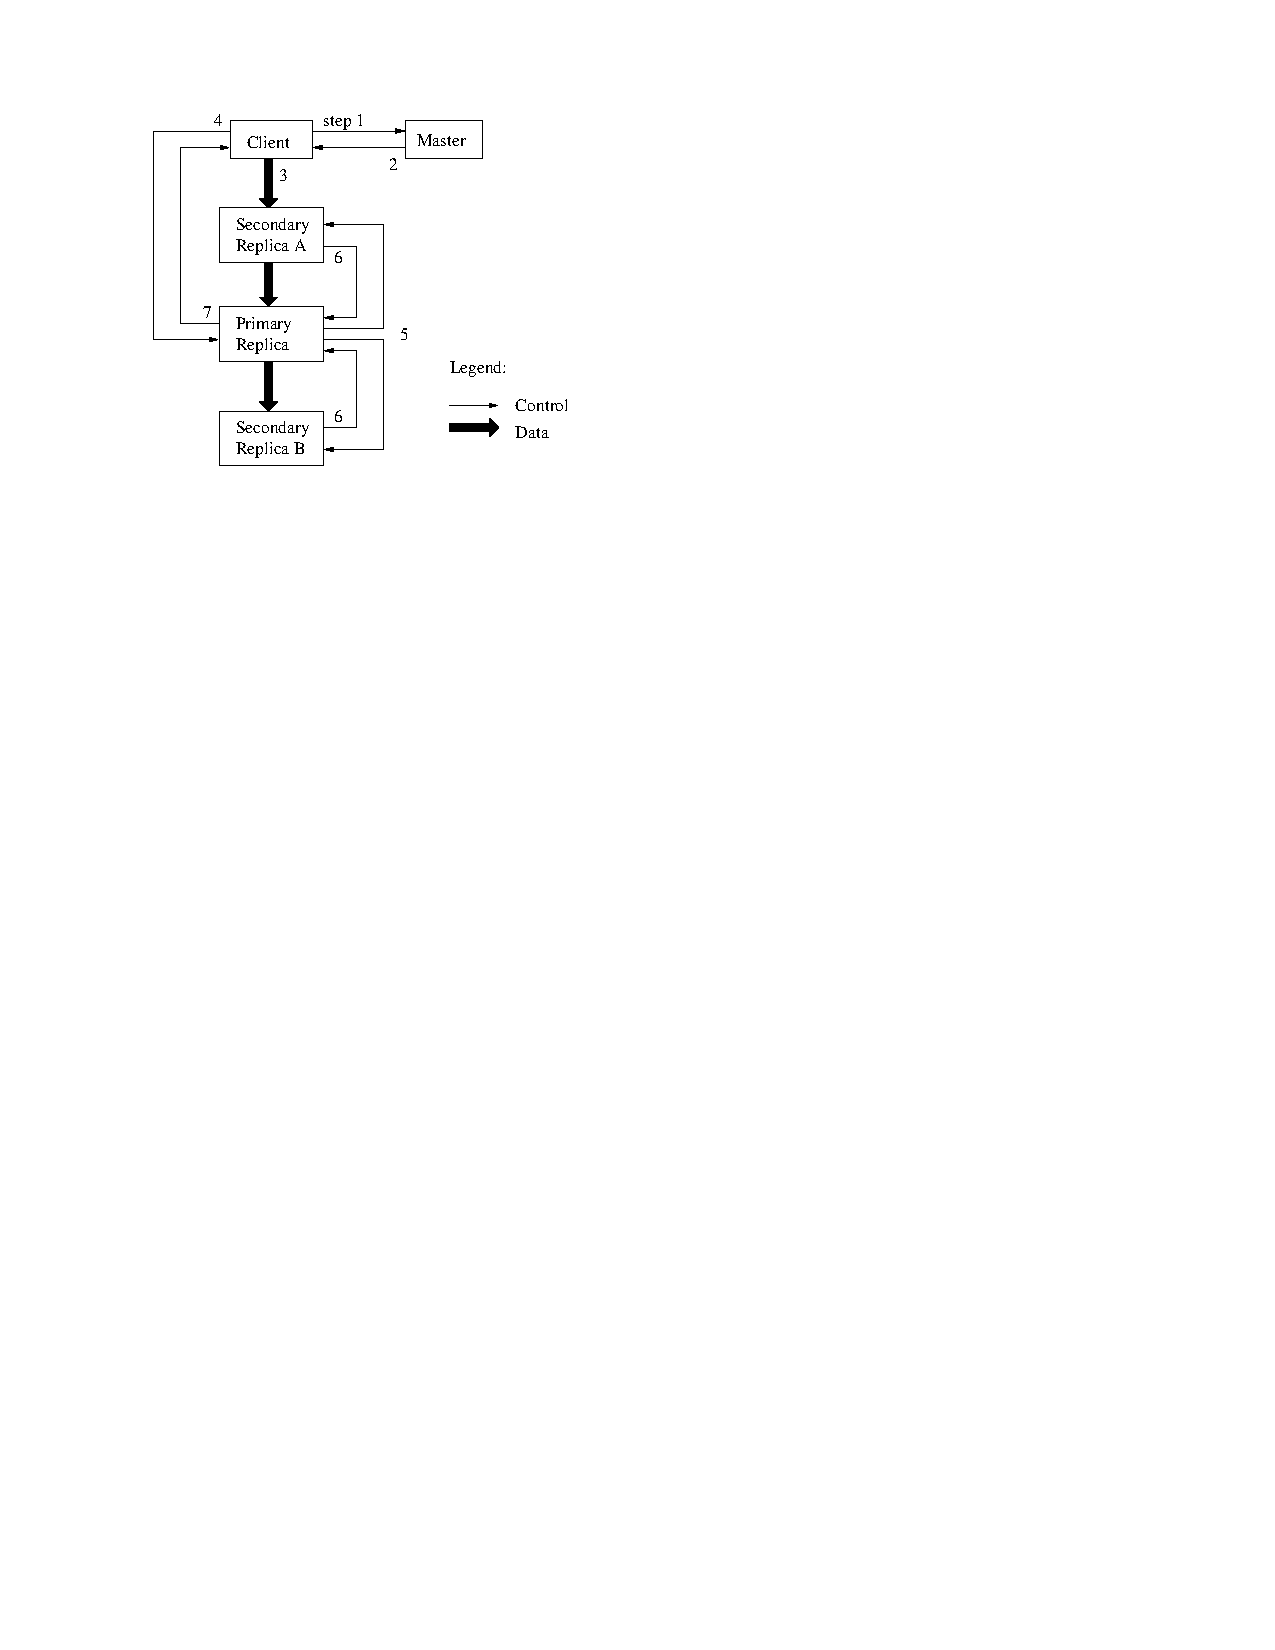
\includegraphics[width=0.45\textwidth]{process}
        \caption{Write Control and Data Flow}
        \label{fig:writecontrol}
\end{figure}

그림 \ref{fig:writecontrol}에서 보여주고 있는 이러한 제어 흐름의 주요 단계를 기술하면 다음과 같다.
\be
\ii 클라이언트는 청크에 대한 현재 임대와 다른 복제본들의 위치를 가지고 있는 청크서버가 어떤 것인지 마스터에게 물어본다.
만약 임대하고 있는 서버가 하나도 없다면, 마스터는 선택한 복제본의 하나를 임대해 준다.

\ii 마스터는 프라이머리의 식별과 다른 복제본들의 위치를 응답해 준다.
클라이언트는 이 데이터를 향후 뮤테이션을 위해 캐시한다. 이러한 작업은 프라이머리가 도달가능하지(unreachable) 않거나, 더이상 임대를 가지고 있지 않은 경우에 다시 마스터와 컨텍하기 위해서 필요하다.

\ii 클라이언트는 데이터를 모든 복제본들에게 푸쉬한다.
클라이언트 이과정을 임의의 순서로 수행할 수 있다.
각 청크서버는 데이터가 사용되거나 축소될 때까지 초기 LRU 버퍼 캐쉬 내에 있는 데이터를 저장할 것이다.
데이터 흐름을 제어 흐름으로부터 분리함으로써, 어떤 청크서버가 프라이머리인지에 관계없이 네트워크 토폴로지에 근거한 고비용의 데이터 흐름을 스케쥴링함으로써 성능을 향상시킬 수 있다. 

\ii 모든 복제본이 데이터 수신을 확인했다면, 클라이언트는 프라이머리에게 쓰기 요청을 전송한다.
이 요청은 모든 복제본들에게 앞서 전송한 데이터를 식별한다.
프라이머리는 직렬화를 제공하는 다수의 클라이언트로 부터의 요청을 수신 모든 뮤테이션들에게 연속된 일련번호를 할당한다.
이것은 일련 번호 순서인 자신의 지역 상태로 뮤테이션을 적용한다.

\ii 프라이머리는 모든 세컨더리 복제본에게 쓰기 요청을 포워드한다.
각 세컨더리 복제본은 프라이머리로부터 요청받은 순번대로 같은 순서로 뮤테이션을 적용한다.

\ii  세컨더리들은 프라이머리에게 각자 연산이 완료되었음을 응답한다.

\ii 프라이머리는 클라이언트에게 완료되었음을 응답한다. 복제본중 오류가 발생한 것들에 대한 내용도 클라이언트에게 보고한다.
오류의 경우, 쓰기가 프라이머리와 임의의 세컨더리 복제본의 서브셋에서 성공한 경우이다.
만약 프라이머리에서 실패한다면, 일련번호를 지정하지 못하고 포워드한다.
클라이언트 요청은 실패로 간주되고 수정된 영역은 불일치한 상태로 내버려둔다.
클라이언트 코드는 이러한 오류에 대해 뮤테이션을 재시도함으로써 처리한다.
쓰기 시작점에서의 재시도를 대신하기 전에 3단계에서 7단계까지를 몇번 시도하게 된다
\ee

\section{Summary}
GFS는 엄청나게 많은 데이터를 보유해야 하는 구글의 핵심 데이터 스토리지와 구글 검색 엔진을 위해 최적화 되었다.
구글 초창기에 래리 페이지와 세르게이 브린에 의해 개발된 “빅파일”에서 개선된 것이다. 
파일들은 일반적인 파일 시스템에서의 클러스터들과 섹터들과 비슷하게 64MB로 고정된 크기의 청크들로 나뉜다. 
이것들은 덮어쓰거나 크기를 줄이는 경우가 극히 드물며 보통 추가되거나 읽혀지기만 한다. 
가격이 저렴한 범용 컴퓨터들로 구성되고 집적도가 높은 구글의 컴퓨팅 클러스터들에서 잘 동작하도록 최적화 되었다. 
가격이 저렴한 서버에서도 사용되도록 설계되었기 때문에 하드웨어 안정성이나 자료들의 유실에 대해서 고려하여 설계되었고 지연시간(latency)이 조금 길더라도 데이터의 높은 처리량(throughput)에 중점을 두었다.


\bibliographystyle{abbrv}
\bibliography{sqlonhadoop}

\end{document}
